% Autogenerated translation of README.md by Texpad
% To stop this file being overwritten during the typeset process, please move or remove this header

\documentclass[12pt]{book}
\usepackage{graphicx}
\usepackage{fontspec}
\usepackage[utf8]{inputenc}
\usepackage[a4paper,left=.5in,right=.5in,top=.3in,bottom=0.3in]{geometry}
\setlength\parindent{0pt}
\setlength{\parskip}{\baselineskip}
\setmainfont{Helvetica Neue}
\usepackage{hyperref}
\pagestyle{plain}
\begin{document}

\chapter*{QChat-An Online Chat Based On UDP\&WebSockets By QT}

\section*{Feature}

Basic Feature of IM
Designed UI
LAN Scan \& Find
Database on Server Support(Pymongo)
Web Chat (Based on WebSockets Server)

\section*{Screenshots}

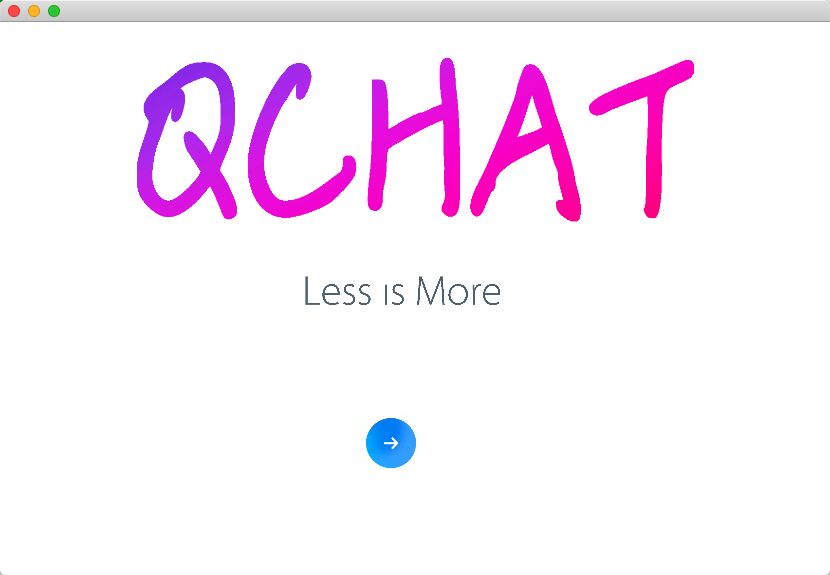
\includegraphics{README/53ACD6E0-0472-420B-946B-15CEDE6D4033.png}

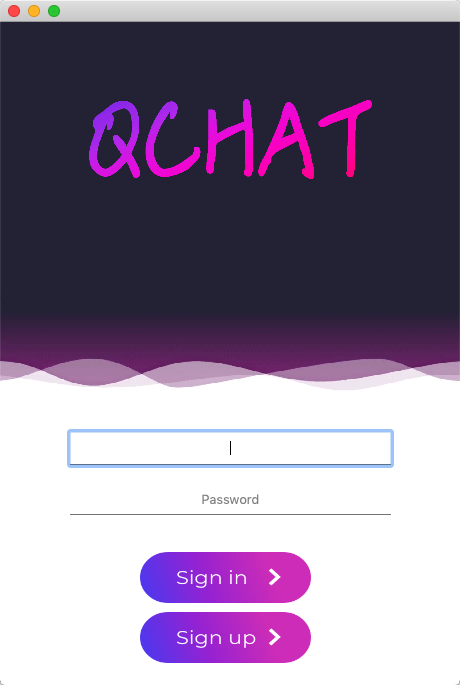
\includegraphics{README/825832A6-C382-4756-B6F6-4BCB18C60C0A.png}

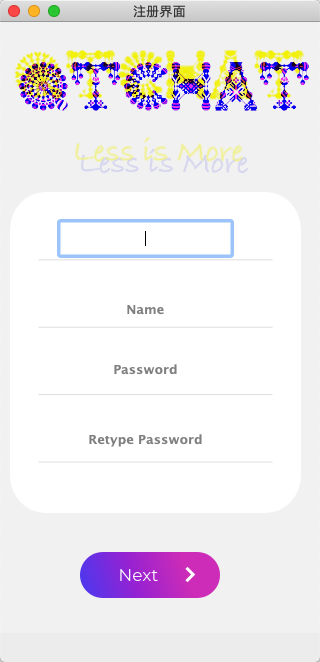
\includegraphics{README/F8E50FED-81F6-4709-8231-464930813F40.png}

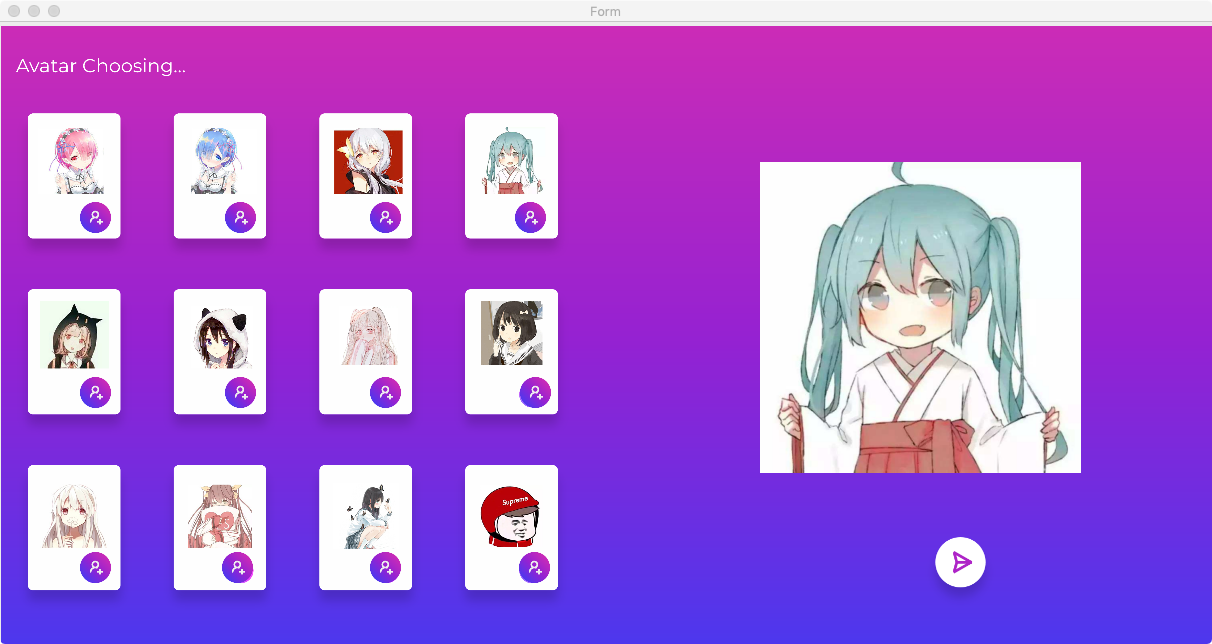
\includegraphics{README/FE90AA8A-2DF4-4867-835B-C852A53228D4.png}

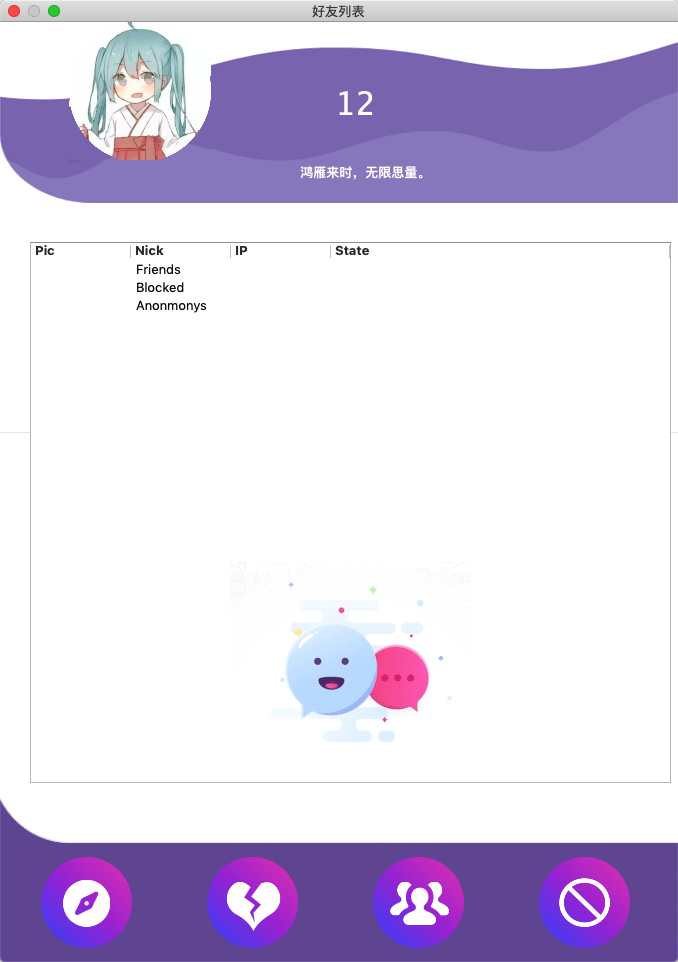
\includegraphics{README/01B83BA9-7C4E-41D7-8AD6-6C0FCCB123C0.png}
(Most of the credit for our impressive UI must go to Yupotian)

\section*{Something You NEED To Know…..}

\begin{enumerate}
\item 本项目为UPC 小学期结课作业,所以可能部分功能并没有实际用途,欢迎二次修改。
\item 严格禁止将本项目或部分功能直接用于(包括但不限于)作业,评比等用途。
\item 本项目的账户功能基于服务器端数据库,因此你需要先行部署服务端并修改服务端IP才能实现注册登录,也欢迎将其修改为基于本地文件版本,将对应位置代码注释取消即可。
\item 服务端基于Python上Flask框架,Flask-Sockets及Pymongo插件,请确认安装了依赖及MongoDB。
\item 欢迎Issue及Pull Request。
\end{enumerate}

\end{document}
